\begin{frame}{Konstrukcija pravokotnice na premico $p$ skozi točko $T$}

	\begin{columns}

		\column{0.55\textwidth}
			\begin{itemize}
				\item<1-> Dani sta premica $p$ in točka $T$.
				\item<2-> Nariši lok $k$ s središčem v $T$.
				\item<3-> Premico $p$ seče v točkah $A$ in $B$.
				\item<4-> Nariši lok $m$ s središčem v $A$.
				\item<5-> Nariši lok $n$ s središčem v $B$ in z enakim polmerom.
				\item<6-> Loka se sečeta v točki $C$.
				\item<7> Premica skozi točki $T$ in $C$ je pravokotna na $p$.
			 \end{itemize}

		\column{0.45\textwidth}
		\centering
		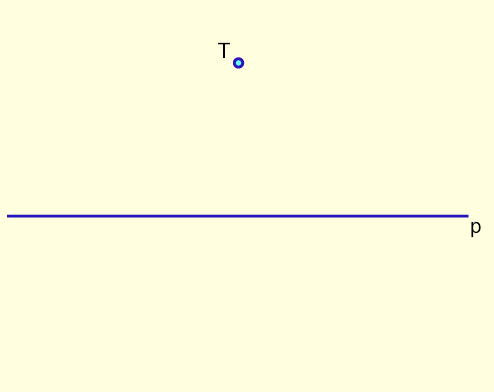
\includegraphics[width=50mm]{slike/fig-1.png}<1>
		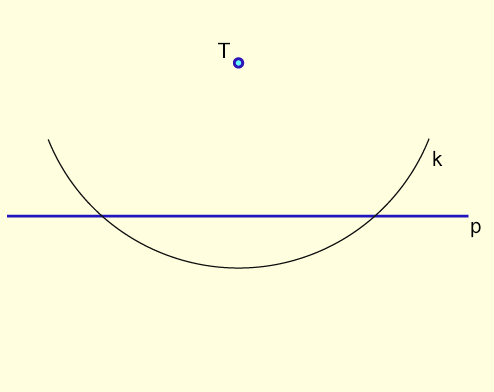
\includegraphics[width=50mm]{slike/fig-2.png}<2>
		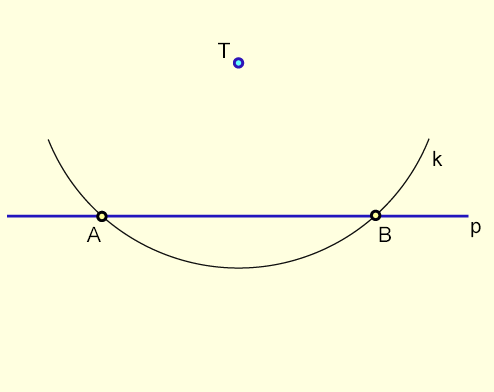
\includegraphics[width=50mm]{slike/fig-3.png}<3>
		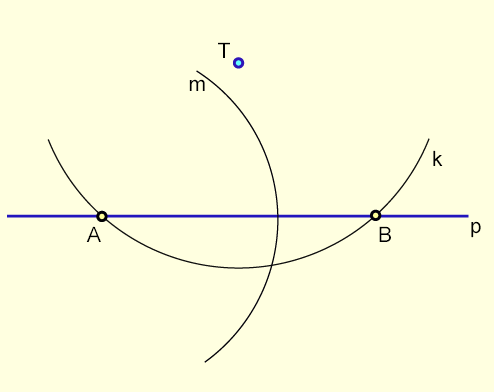
\includegraphics[width=50mm]{slike/fig-4.png}<4>
		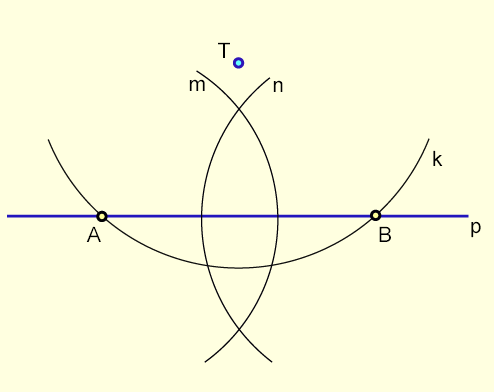
\includegraphics[width=50mm]{slike/fig-5.png}<5>
		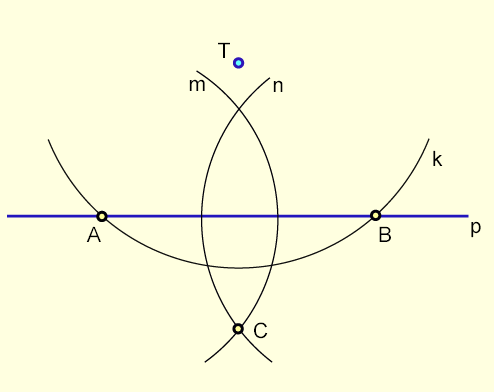
\includegraphics[width=50mm]{slike/fig-6.png}<6>
		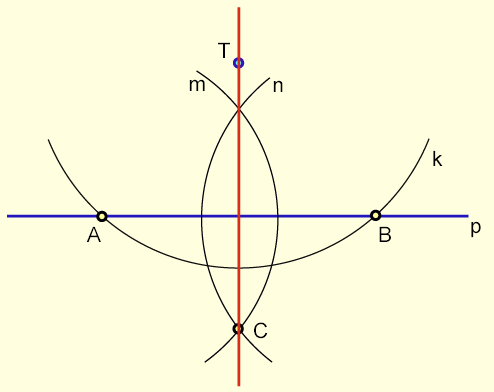
\includegraphics[width=50mm]{slike/fig-7.png}<7>
	\end{columns}
	
	
\end{frame}

\begin{frame}{Konstrukcija pravokotnice na premico $p$ skozi točko $T$}

	\begin{columns}

		\column{0.55\textwidth}
			\begin{itemize}
				\item<1-> Dani sta premica $p$ in točka $T$.
				\item<2-> Nariši lok $k$ s središčem v $T$.
				\item<3-> Premico $p$ seče v točkah $A$ in $B$.
				\item<4-> Nariši lok $m$ s središčem v $A$.
				\item<5-> Nariši lok $n$ s središčem v $B$ in z enakim polmerom.
				\item<6-> Loka se sečeta v točki $C$.
				\item<7> Premica skozi točki $T$ in $C$ je pravokotna na $p$.
			 \end{itemize}
		
		\column{0.44\textwidth}
		% Spodnje je za nalogo 3.4.

				 % Sliko smo naredili tako, da so točke A, B, T in C vse enako oddaljene
				 % od presečišča premic; kot ATC je 45°.
				 % Vsi krožni loki imajo radij 2.
				 \begin{tikzpicture}
				 \tikzmath{
				 	% Razdalja od točke T do premice p je tako 2*sin(45°).
				 	\t = 2*sin(45);
				 	% Razdalja začetka loka m do premice p
				 	% oz. razdalja točke T' levo in zgoraj od točke T do premice
				 	\tt = 2*sin(60);
				 	% Razdalja točke T' od navpične premice skozi T
				 	\td = \t-2*cos(60);
				 }
				 \only{\draw[red, very thick] (0,-2) -- (0,2) node[right] {};}<7>
				 % Definicija točke T
				 \coordinate [label={[blue, above left]:$T$}] (T) at (0,{\t});
				 % Risanje točke T
				 \fill[blue] (T) circle (2pt);
				 % Premica p
				 \draw[blue, very thick] (-2,0) -- (2,0) node[right] {$p$};
				 \pause
				 % Definicija pomožne točke A' in risanje krožnega loka k, ki se začne v A'
				 \coordinate (A') at ({-\tt},{\td});
				 \draw[gray, thin] (A') arc[start angle=210, end angle=330, radius=2] node[right] {\scriptsize $k$};
				 \pause
				 % Točka A
				 \coordinate [label=below left:{\scriptsize $A$}] (A) at ({-\t},0);
				 \draw (A) circle (1.5pt);
				
				 % Naloga 3.4.1.: Narišite še točko B (skupaj z oznako)
				 \coordinate [label=below right:{\scriptsize $B$}] (B) at ({\t},0);
				 \draw (B) circle (1.5pt);
				 \pause
				 % Naloga 3.4.2.: Definirajte točko T', v kateri se začne lok m in narišite lok m z oznako.
				 \coordinate (T') at ({-\td},{-\tt});
				 \draw[gray, thin] (T') arc[start angle=-60, end angle=60, radius=2] node[below left] {\scriptsize $m$};
				 \pause
				 % Lok je definiran s točko, v kateri se lok začne (ne središče!), z začetnim in končnim kotom ter radijem.
				 % Koti so vedno podani enako: kot 0 je v smeri x osi in se veča v nasprotni smeri urinega kazalca.

				 % Naloga 3.4.3.: Definirajte točko T'' in narišite lok n z oznako.
				 \coordinate (T'') at ({\td},{-\tt});
				 \draw[gray, thin] (T'') arc[start angle=240, end angle=120, radius=2] node[below right] {\scriptsize $n$};
				 \pause
				 % Naloga 3.4.4.: Definirajte in narišite točko C.
				 \coordinate [label=below right:{\scriptsize $C$}] (C) at (0,{-\t});
				 \draw (C) circle (1.5pt);
				 \pause
				 % Naloga 3.4.5.: Narišite premico skozi točki T in C.
				% Konec vsebine za nalogo 3.4.
			\end{tikzpicture}
	\end{columns}
	
	
\end{frame}

				


% Naloga 4
\begin{frame}{Graf funkcije s TikZ}
	\centering
	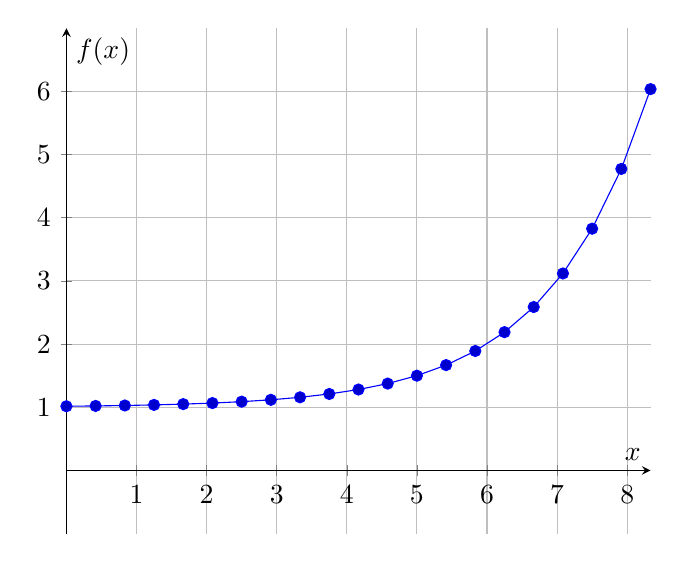
\begin{tikzpicture}
		\begin{axis}[
			axis lines = middle,
			xlabel = {$x$},
			ylabel = {$f(x)$},
			width = 9cm,
			height = 8cm,
			grid = both,
			domain = 0:10,
			xtick = {0, 1, 2, 3, 4, 5, 6, 7, 8},
			ytick = {0, 1, 2, 3, 4, 5, 6},
			ymin = -1,
			ymax = 7
			]
		\addplot{2^(x - 3)/2^3 + 1};
		\end{axis}
	\end{tikzpicture}
\end{frame}